\chapter{La suma de convolución}

\section{Deducción de la fórmula}

A continuación calculamos la salida $y[n]$ de un sistema lineal para una entrada arbitraria $x[n]$. Para poder hacerlo, usamos pulsos desplazados en el tiempo $\delta[n-n_{0}]$ donde $n_{0}$ es un instante de tiempo.

\subsection{Representación de señales en términos de impulsos}

\begin{enumerate}
	
	\item Consideremos una secuencia $x[n]$ (ver Fig. \ref{fig:convone}). Por la propiedad del muestreo podemos escribir:
	\begin{align}
		x[-2]\delta[n+2] &= \begin{cases}
			x[-2], & n=-2, \\ 
			0,     & n\neq -2.
		\end{cases} \\
		x[-1]\delta[n+1] &= \begin{cases}
			x[-1], & n=-1, \\ 
			0,     & n\neq -1.
		\end{cases} \\
		x[0]\delta[n] &= \begin{cases}
			x[0], & n=0, \\ 
			0,    & n\neq 0.
		\end{cases} \\
		x[1]\delta[n-1] &= \begin{cases}
			x[1], & n=1, \\ 
			0,    & n\neq 1.
		\end{cases} \\
		x[2]\delta[n-2] &= \begin{cases}
			x[2], & n=2, \\ 
			0,    & n\neq 2.
		\end{cases}
	\end{align}
	y en general:
	\begin{equation}
		x[k]\delta[n-k] = \begin{cases}
			x[k], & n=k, \\ 
			0,    & n\neq k.
		\end{cases}
	\end{equation}
	
	\item Como podemos ver en la Fig. (\ref{fig:convone}), la suma de impulsos desplazados en el tiempo multiplicados por coeficientes adecuados equivalen a cualquier señal arbitraria $x[n]$.
	
	\begin{figure}[htbp]
		\centering
		\includegraphics[width=3in]{./graphics/convone.png}
		\caption{Una señal como suma de impulsos desplazados en el tiempo multiplicados por coeficientes adecuados. Los impulsos desplazados $\delta[n-k]$ se representan $d[n-k]$. Sólo se muestran tres impulsos por razones de espacio.}
		\label{fig:convone}
	\end{figure}
	
	\item En efecto, agregando más impulsos desplazados y multiplicados adecuadamente podemos obtener una expresión que se puede escribir en forma general:
	\begin{equation}
		x[n] = \sum_{k=-\infty}^{\infty} x[k] \, \delta[n-k].
		\label{cduna.5}
	\end{equation}
	
	\item La Ec. (\ref{cduna.5}) corresponde a la representación de una secuencia arbitraria $x[n]$ como:
	\begin{itemize}
		\item una combinación lineal de impulsos desplazados $\delta[n-k]$,
		\item donde los coeficientes de la combinación lineal son los valores $x[k]$.
	\end{itemize}
	
	\item Cada impulso desplazado $\delta[n-k]$ actúa como selector: suponga que elegimos un valor $n=n_{0}$ y entonces tenemos que:
	\begin{equation}
		x[n_{0}] = \sum_{k=-\infty}^{\infty} x[k] \, \delta[n_{0}-k].
		\label{cddos.5}
	\end{equation}
	
	\item Recordemos la definición de impulso:
	\begin{equation}
		\delta[n] = \begin{cases}
			1, & n=0, \\ 
			0, & n\neq 0.
		\end{cases}
	\end{equation}
	El impulso ``vale'' $1$ cuando el índice $n$ (lo que aparece entre corchetes) vale $0$. Note que en la ec. (\ref{cddos.5}) sólo uno de los infinitos impulsos tiene un índice nulo, específicamente:
	\begin{equation}
		n_{0}-k=0.
	\end{equation}
	Entonces, de todos los infinitos términos sólo uno es no nulo ($k=n_{0}$). Así obtenemos la igualdad:
	\begin{equation}
		x[n_{0}] = x[n_{0}].
	\end{equation}
	
	\item La utilidad de la ecuación (\ref{cduna.5}) es que expresa una secuencia
	\begin{equation}
		...x[-3], \, x[-2], \, x[-1], \, x[0], \, x[1], \, x[2], \, x[3]...
	\end{equation}
	como una sumatoria.
\end{enumerate}

\subsection{La respuesta al impulso y la suma de convolución}

\begin{enumerate}
	
	\item Sea $h_{k}[n] = h[n-k]$ la respuesta de un sistema lineal $S$ al impulso unitario desplazado $\delta[n-k]$,
	\begin{align*}
		\vdots & \\ 
		\delta[n+1] &\xrightarrow{S} h_{-1}[n], \\ 
		\delta[n] &\xrightarrow{S} h_{0}[n], \\ 
		\delta[n-1] &\xrightarrow{S} h_{1}[n], \\ 
		\vdots & \\ 
		\delta[n-k] &\xrightarrow{S} h_{k}[n].
	\end{align*}
	Vea la Fig. (\ref{fig:convtwoone}).
	\begin{figure}[htbp]
		\centering
		\includegraphics[width=3in]{./graphics/convtwoone.png}
		\caption{Las respuestas de un sistema lineal frente a impulsos desplazados en el tiempo. Los gráficos de la columna izquierda representan las entradas, y los de la columna derecha las salidas.}
		\label{fig:convtwoone}
	\end{figure}
	
	\item Como el sistema $S$ es lineal, podemos multiplicar a ambos lados por constantes y obtenemos:
	\begin{align*}
		\vdots & \\ 
		x[-1] \delta[n+1] &\xrightarrow{S} x[-1] h_{-1}[n], \\ 
		x[0] \delta[n] &\xrightarrow{S} x[0] h_{0}[n], \\ 
		x[1] \delta[n-1] &\xrightarrow{S} x[1] h_{1}[n], \\ 
		\vdots & \\ 
		x[k] \delta[n-k] &\xrightarrow{S} x[k] h_{k}[n].
	\end{align*}
	Como el sistema es lineal, podemos ``sumar'' las infinitas entradas y las infinitas salidas para obtener:
	\begin{equation}
		x[n] = \left( \sum_{k=-\infty}^{\infty} x[k] \delta[n-k] \right) 
		\xrightarrow{S}
		\left( \sum_{k=-\infty}^{\infty} x[k] h_{k}[n] \right) = y[n].
		\label{convo}
	\end{equation}
	Vea la Fig. (\ref{fig:convtwotwo}).
	
	\begin{figure}[htbp]
		\centering
		\includegraphics[width=3in]{./graphics/convtwotwo.png}
		\caption{En la columna de la izquierda, desde la primera a la quinta fila vemos impulsos desplazados en el tiempo $\delta[n-k]$ multiplicados por $x[k]$. En la columna de la derecha, en las filas respectivas vemos las respuestas correspondientes. En los subgráficos de la sexta fila, vemos la suma de los resultados parciales para obtener la señal de entrada $x[n]$ (izquierda) y la salida correspondiente $y[n]$ (derecha).}
		\label{fig:convtwotwo}
	\end{figure}
	Por el principio de superposición, $y[n]$ es la respuesta a la entrada $x[n]$:
	\begin{equation}
		y[n] = \sum_{k=-\infty}^{\infty} x[k] h_{k}[n]
	\end{equation}
	
	\item Si el sistema $S$ es invariante en el tiempo, entonces para cualquier valor de $k$ se cumple que:
	\begin{equation}
		h_{k}[n] = h_{0}[n].
	\end{equation}
	Por conveniencia notacional, definimos la respuesta al impulso de un sistema invariante en el tiempo:
	\begin{equation}
		h[n] = h_{0}[n],
	\end{equation}
	o sea que $h[n]$ es la salida de un sistema $S$ LTI cuando $\delta[n]$ es la entrada. Entonces podemos escribir:
	\begin{equation}
		h_{k}[n] =  h[n-k],
	\end{equation}
	y
	\begin{equation}
		y[n] = \sum_{k=-\infty}^{\infty} x[k] h[n-k].
	\end{equation}
	Esta es la suma de convolución o superposición. La convolución de dos señales se representa:
	\begin{equation}
		y[n] = x[n] * h[n].
	\end{equation}
	
\end{enumerate}

\section{Ejemplos}

\subsection{Convolución con un impulso desplazado}

Supongamos un sistema con una respuesta al impulso $h[n] = \delta[n - n_{0}]$. Vamos a calcular su salida para una entrada $x[n]$.

\begin{enumerate}
	\item Comenzamos escribiendo la suma de convolución:
	\begin{equation}
		y[n] = \sum_{k=-\infty}^{\infty} x[k] h[n-k].
	\end{equation}
	\item Si $h[n] = \delta[n - n_{0}]$, entonces $h[n - k] = \delta[n - n_{0} - k]$.
	\item Reemplazando $h[n - k]$ en la suma de convolución resulta:
	\begin{equation}
		y[n] = \sum_{k=-\infty}^{\infty} x[k] h[n-k] = \sum_{k=-\infty}^{\infty} x[k] \delta[n - n_{0} - k].
	\end{equation}
	Observemos que tenemos una señal $x[k]$ multiplicada por un impulso $\delta[n - n_{0} - k]$.
	\item ¿Dónde ``vale'' $1$ el impulso $\delta[n - n_{0} - k]$? Justo cuando $n - n_{0} - k = 0$.
	\item ¿Para cuál valor de $k$ la señal $x[k]$ va a estar multiplicada por $1$, y para cuáles valores de $k$ va a estar multiplicada por $0$?
	\item Para el valor $k = n - n_{0} \implies x[k] \, \delta[n - n_{0} - k] = x[n - n_{0}] \, \delta[0]$.
	\item Para los valores $n - n_{0} - k = m \neq 0$ se verifica:
	\begin{equation}
		x[k] \, \delta[n - n_{0} - k] = x[n - n_{0} - m] \cdot 0 = 0.
	\end{equation}
	\item Por lo tanto:
	\begin{equation}
		y[n] = \dots + x[n - n_{0} + 1] \cdot 0 + x[n - n_{0}] \cdot 1 + x[n - n_{0} - 1] \cdot 0 + \dots 
	\end{equation}
	\item El resultado es:
	\begin{equation}
		y[n] = \sum_{k=-\infty}^{\infty} x[k] h[n-k] = x[n - n_{0}].
	\end{equation}
	\item Como la respuesta al impulso es un impulso desplazado en el tiempo, todas las entradas para este sistema generan salidas desplazadas en el tiempo.
\end{enumerate}

\subsection{Convolución con varios impulsos desplazados}

Supongamos que tenemos un sistema lineal invariante en el tiempo con respuesta al impulso $h[n] = \delta[n - n_{0}] + \delta[n - n_{1}]$. Calcular la respuesta $y[n]$ para una entrada $x[n]$.

\begin{enumerate}
	\item Si la respuesta al impulso fuera $h[n] = \delta[n - n_{0}]$, la salida sería $y[n] = x[n - n_{0}]$.
	\item Si la respuesta al impulso fuera $h[n] = \delta[n - n_{1}]$, la salida sería $y[n] = x[n - n_{1}]$.
	\item Entonces, para $h[n] = \delta[n - n_{0}] + \delta[n - n_{1}]$, la salida es $y[n] = x[n - n_{0}] + x[n - n_{1}]$ (Principio de superposición).
\end{enumerate}

\section{La suma de convolución paso a paso}

Para calcular la convolución 
\begin{equation}
	y[n] = \sum_{k=-\infty}^{\infty} x[k] h[n - k],
\end{equation}
en el momento $n = n_{0}$, debemos ejecutar los siguientes pasos:
\begin{enumerate}
	\item reemplazar la variable independiente $k$ por $-k$ para obtener $h[-k]$, la versión reflejada respecto a $k = 0$.
	\item desplazar $h[-k]$ a la posición $n_{0}$, o en otras palabras, se desplaza $h[-k]$ de forma tal que el valor original $h[0]$ esté ubicado en $k = n_{0}$.
	\item evaluar el producto $z[n_{0},k] = x[k] \, h[n_{0} - k]$.
	\item evaluar la sumatoria $y[n_{0}] = \sum_{k=-\infty}^{\infty} z[n_{0},k]$.
\end{enumerate}

\section{Cálculo de la suma de convolución en forma gráfica}

El cálculo de la convolución tiene una interpretación gráfica.
\begin{enumerate}
	\item Consideremos la fórmula:
	\begin{equation}
		y[n] = \sum_{k=-\infty}^{\infty} x[k] h[n-k].
		\label{condiscgraf}
	\end{equation}
	
	\item En la ec. (\ref{condiscgraf}) el factor $h[n-k]$ es una versión de $h[k]$ invertida en el tiempo (observe la variable $k$ en ambas funciones) y desplazada en el tiempo (observe la variable $n$, que toma un valor constante para todos los sumandos $x[k] h[n-k]$).
	\item En la ec. (\ref{condiscgraf}), el desplazamiento en el tiempo del factor $h[n-k]$ depende del índice de la salida $y[n]$.
	\item En base a las anteriores observaciones, es posible enunciar la siguiente ``receta'' para calcular la convolución en forma gráfica:
	\begin{enumerate}
		\item Dibuje la señal $x[k]$.
		\item Invierta en el tiempo la señal $h[k]$ para obtener $h[-k]$.
		\item Repita los siguientes pasos para calcular distintos valores de $y[n]$:
		\begin{enumerate}
			\item Desplace en el tiempo la señal $h[-k]$ para obtener $h[n-k]$.
			\item Obtenga el producto $z[n,k] = x[k] \, h[n-k]$.
			\item El valor de $y[n]$ es $\sum_{k} z[n,k]$.
		\end{enumerate}
	\end{enumerate}
\end{enumerate}

\section{Ejemplos}

\subsection{Convolución de señales de duración finita}

Calculemos la convolución de las señales:
\begin{align}
	x[n] &= \begin{cases}
		2, & n=1, \\ 
		-2, & n=2, \\ 
		0, & \text{resto}.
	\end{cases} \\ 
	h[n] &= \begin{cases}
		-1, & n=1, \\ 
		-1, & n=2, \\ 
		0, & \text{resto}.
	\end{cases}
\end{align}

Dado que podemos considerar la señal $x[n]$ como dos impulsos desplazados y multiplicados por coeficientes, podemos calcular las respuestas del sistema a los impulsos por separado y sumarlas después de multiplicarlas por los coeficientes adecuados. Tenemos entonces:

\begin{center}
	\begin{tabular}{ccccc}
		$n$ &  $h[n-1]$ & $h[n-2]$ & $y[n] = h[n-1] x[1] + h[n-2] x[2]$ \\ \hline
		$0$ &  $0$      & $0$      & $0$  \\
		$1$ &  $0$      & $0$      & $0$  \\
		$2$ &  $-1$     & $0$      & $-2$ \\
		$3$ &  $-1$     & $-1$     & $0$  \\
		$4$ &  $0$      & $-1$     & $2$  \\
		$5$ &  $0$      & $0$      & $0$  \\
		$6$ &  $0$      & $0$      & $0$
	\end{tabular}
\end{center}

Resumiendo:
\begin{equation}
	y[n] = \begin{cases}
		-2, & n=2, \\ 
		0,  & n=3, \\ 
		2,  & n=4, \\ 
		0,  & \text{resto}.
	\end{cases}
\end{equation}

\subsubsection{Forma gráfica}

\begin{enumerate}
	\item Dibujemos las señales $x[n]$, $h[n]$ y $h[-n]$. Ver Fig. (\ref{fig:convejemp0101}) a (\ref{fig:convejemp0106}).
	\item Dibujemos $h[n-k]$ para distintos valores de $n$, junto con $x[k]$.
	\item Dibujemos el producto $z[n,k] = x[k] \, h[n-k]$.
	\item Calculemos $\sum_{k}z[n,k]$ para obtener $y[n]$.
\end{enumerate}

\begin{figure}[htbp]
	\centering
	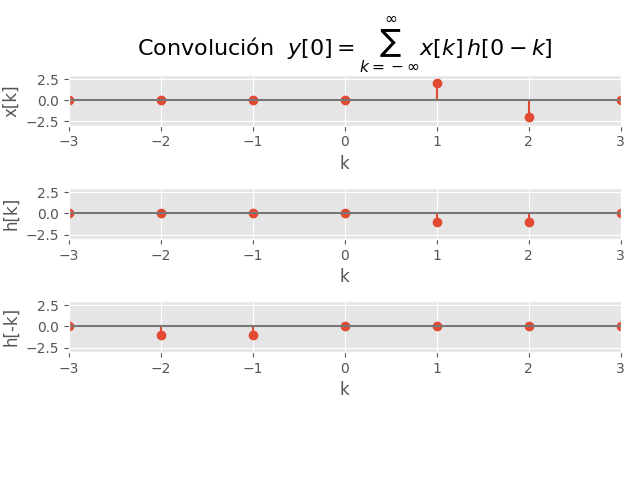
\includegraphics[width=6in]{./graphics/convejemp01-01.png}
	\caption{Señales $x[k]$, $h[k]$ y $h[-k]$.}
	\label{fig:convejemp0101}
\end{figure}

\begin{figure}[htbp]
	\centering
	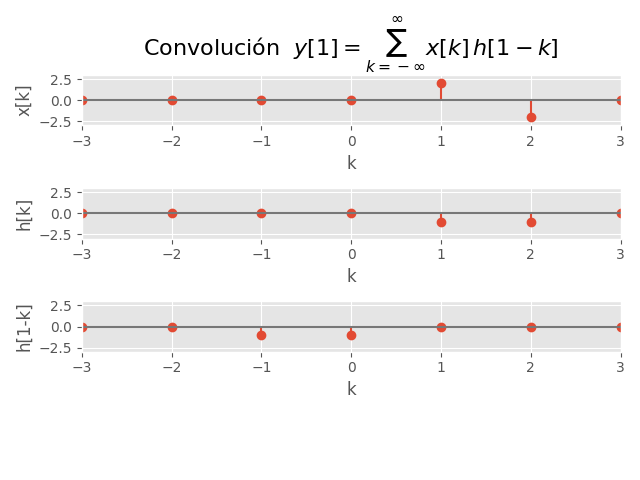
\includegraphics[width=6in]{./graphics/convejemp01-02.png}
	\caption{Señales $x[k]$, $h[k]$ y $h[1-k]$.}
	\label{fig:convejemp0102}
\end{figure}

\begin{figure}[htbp]
	\centering
	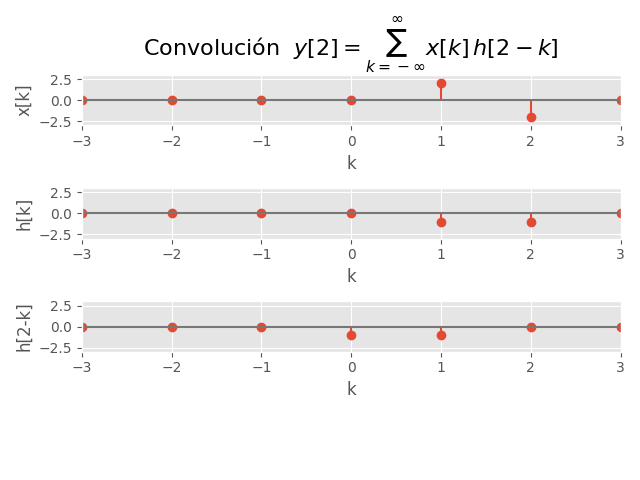
\includegraphics[width=6in]{./graphics/convejemp01-03.png}
	\caption{Señales $x[k]$, $h[k]$ y $h[2-k]$.}
	\label{fig:convejemp0103}
\end{figure}

\begin{figure}[htbp]
	\centering
	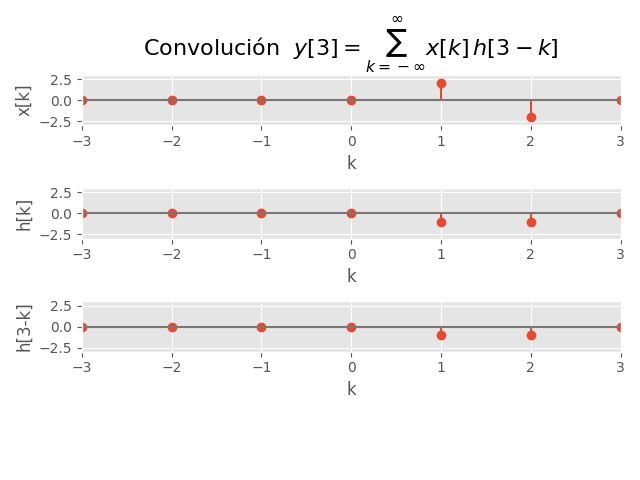
\includegraphics[width=6in]{./graphics/convejemp01-04.png}
	\caption{Señales $x[k]$, $h[k]$ y $h[3-k]$.}
	\label{fig:convejemp0104}
\end{figure}

\begin{figure}[htbp]
	\centering
	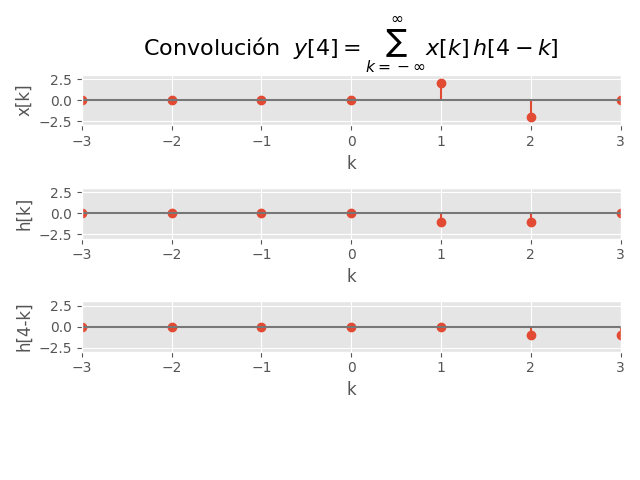
\includegraphics[width=6in]{./graphics/convejemp01-05.png}
	\caption{Señales $x[k]$, $h[k]$ y $h[4-k]$.}
	\label{fig:convejemp0105}
\end{figure}

\begin{figure}[htbp]
	\centering
	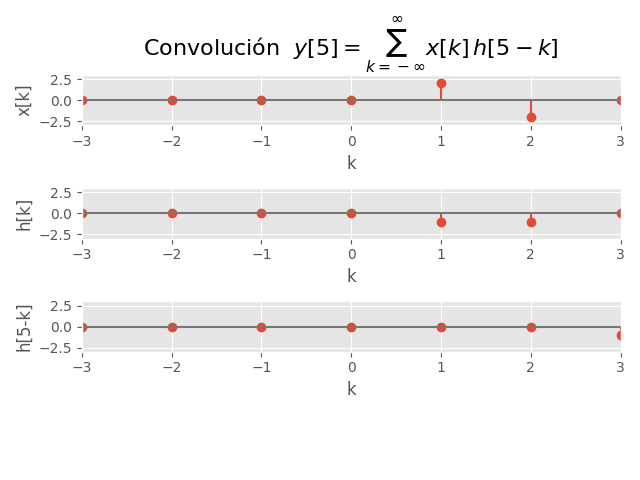
\includegraphics[width=6in]{./graphics/convejemp01-06.png}
	\caption{Señales $x[k]$, $h[k]$ y $h[5-k]$.}
	\label{fig:convejemp0106}
\end{figure}

\subsection{Convolución con un impulso}

Calculemos ahora la convolución de las señales:
\begin{align}
	x[n] &= \left( \frac{99}{100}\right)^n u[n], \\
	h[n] &= \delta[n-1].
\end{align}

\subsubsection{Forma gráfica}

\begin{enumerate}
	\item Dibujemos las señales $x[k]$, $h[k]$ y $h[-k]$.
	\item Dibujemos $h[n-k]$ para distintos valores de $n$, junto con $x[k]$. Ver Fig. (\ref{fig:convejemp0201}).
	\item Dibujemos el producto $z[n,k] = x[k] \, h[n-k]$.
	\item Calculemos $\sum_{k}z[n,k]$ para obtener $y[n]$.
\end{enumerate}

\begin{figure}[htbp]
	\centering
	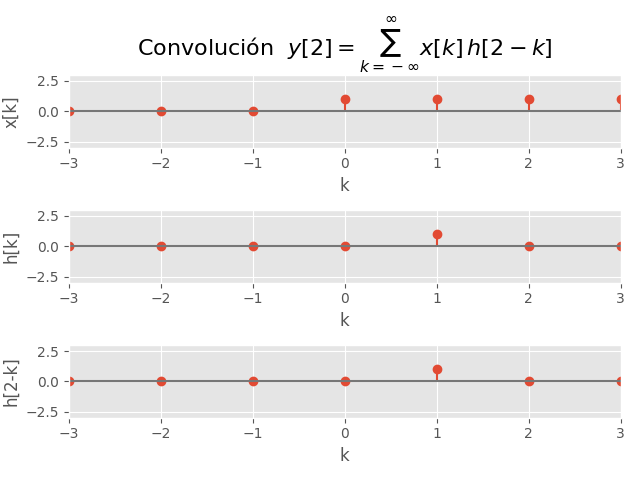
\includegraphics[width=6in]{./graphics/convejemp02-01.png}
	\caption{Señales $x[k]$, $h[k]$ y $h[2-k]$.}
	\label{fig:convejemp0201}
\end{figure}

\subsubsection{Forma analítica}

\begin{enumerate}
	\item Según la Ec. (\ref{convo}), tenemos:
	\begin{equation}
		y[n] = \sum_{k=-\infty}^{\infty} \left( \frac{99}{100}\right)^k u[k] \, \delta[n-1-k].
	\end{equation}
	
	\item Dado que dentro de la sumatoria aparece un escalón unitario, podemos eliminarlo modificando adecuadamente el límite inferior del índice $k$. Además, dado que la entrada contiene un factor escalón $u[n]$, la salida también tiene un factor similar. Entonces, como $u[k] = 0$ para $k < 0$, el límite inferior es $k = 0$, y además la sumatoria queda multiplicada por $u[n]$:
	\begin{equation}
		y[n] = \left(\sum_{k=0}^{\infty} \left( \frac{99}{100}\right)^k \delta[n-1-k] \right) \cdot u[n].
		\label{ejeconvimpulso.0}
	\end{equation}
	
	\item Observe que el índice del impulso es $n - 1 - k$, y que por lo tanto está ubicado en $k = n - 1$. Entonces:
	\begin{equation}
		\sum_{k=0}^{\infty}\left( \frac{99}{100}\right)^k \delta[n-1-k] = 
		\left( \frac{99}{100}\right)^{n-1} \delta[0] =
		\left( \frac{99}{100}\right)^{n-1}
		\label{ejeconvimpulso}
	\end{equation}
	
	\item Reemplazando (\ref{ejeconvimpulso}) en (\ref{ejeconvimpulso.0}), obtenemos:
	\begin{equation}
		y[n] = \left( \frac{99}{100}\right)^{n-1} \cdot u[n].
	\end{equation}
	
	\item En general, consideremos una respuesta al impulso:
	\begin{equation}
		h[n] = \delta[n-n_{0}].
	\end{equation}
	y calculemos su convolución para una entrada genérica $x[n]$.
	
	\item Según la Ec. (\ref{convo}), tenemos:
	\begin{equation}
		y[n] = \sum_{k=-\infty}^{\infty} x[k] \, \delta[n-n_{0}-k],
	\end{equation}
	
	\item Observe que el índice del impulso es $n - n_{0} - k$, y que por lo tanto está ubicado en $k = n - n_{0}$. Entonces:
	\begin{equation}
		x[k] \, \delta[n-n_{0}-k] = x[n-n_{0}] \, \delta[0] = x[n-n_{0}].
	\end{equation}
	
	\item Considerando la sumatoria, obtenemos:
	\begin{equation}
		\sum_{k=-\infty}^{\infty} x[n-n_{0}] \delta[n-n_{0}-k] = x[n-n_{0}].
	\end{equation}
	
	\item Dado que
	\begin{equation}
		u[n-n_{0}] = \left( \sum_{k=-\infty}^{\infty} \delta[n-n_{0}-k] \right)
	\end{equation}
	la salida $y[n]$ es:
	\begin{equation}
		y[n] = x[n-n_{0}] \, u[n-n_{0}].
	\end{equation}
\end{enumerate}

\subsection{Convolución de una señal con una ventana rectangular}

Calculemos la convolución de las señales:
\begin{align}
	x[n] &= \left( \frac{1}{2}\right)^n u[n], \\
	h[n] &= u[n] - u[n-2] = \delta[n] + \delta[n-1].
\end{align}

\subsubsection{Forma gráfica}

\begin{enumerate}
	\item Dibujemos las señales $x[k]$, $h[k]$ y $h[-k]$.
	\item Dibujemos $h[n-k]$ para distintos valores de $n$, junto con $x[k]$.
	\item Dibujemos el producto $z[n,k] = x[k] h[n-k]$.
	\item Calculemos $\sum_{k}z[n,k]$ para obtener $y[n]$.
\end{enumerate}

\subsubsection{Forma analítica}

\begin{enumerate}
	\item Según la Ec. (\ref{convo}), tenemos:
	\begin{equation}
		y[n] = \sum_{k=-\infty}^{\infty} \left( \frac{1}{2}\right)^k u[k] \, h[n-k].
	\end{equation}
	
	\item Ajustamos los índices de la sumatoria porque la señal es nula para $k < 0$:
	\begin{equation}
		y[n] = \sum_{k=0}^{\infty} \left( \frac{1}{2}\right)^k \, h[n-k].
	\end{equation}
	
	\item Expresamos a la ventana rectangular como una suma de impulsos desplazados en el tiempo:
	\begin{equation}
		y[n] = \sum_{k=0}^{\infty} \left( \frac{1}{2}\right)^k \left(\delta[n-k] + \delta[n-1-k] \right).
	\end{equation}
	
	\item Desdoblamos la convolución en dos:
	\begin{align}
		\sum_{k=0}^{\infty} \left( \frac{1}{2}\right)^k \, \delta[n-k] &= \left( \frac{1}{2}\right)^n u[n], \\
		\sum_{k=0}^{\infty} \left( \frac{1}{2}\right)^k \, \delta[n-1-k] &= \left( \frac{1}{2}\right)^{n-1} u[n-1].
	\end{align}
	
	\item El resultado final es:
	\begin{equation}
		y[n] = \left( \frac{1}{2}\right)^n u[n] + \left(\frac{1}{2}\right)^{n-1} u[n-1].
	\end{equation}
\end{enumerate}

\subsection{Convolución de señales infinitas}

Considere una entrada $x[n]$ y una respuesta al impulso unitario dadas por:
\begin{align}
	x[n] &= \alpha^n u[n], \\
	h[n] &= u[n],
\end{align}
donde el valor absoluto de $\alpha$ es menor que $1$:
\begin{equation}
	0 < |\alpha| < 1.
\end{equation}

\subsubsection{Forma gráfica}

\begin{enumerate}
	\item Dibujemos las señales $x[k]$, $h[k]$ y $h[-k]$.
	\item Dibujemos $h[n-k]$ para distintos valores de $n$, junto con $x[k]$.
	\item Dibujemos el producto $z[n,k] = x[k] \, h[n-k]$.
	\item Calculemos $\sum_{k} z[n,k]$ para obtener una aproximación de $y[n]$.
\end{enumerate}

\subsubsection{Forma analítica}

\begin{enumerate}
	\item Según la Ec. (\ref{convo}), tenemos:
	\begin{equation}
		\alpha^{k} u[k] u[n-k] = \begin{cases}
			\alpha^k, & 0 \leq k \leq n, \\ 
			0, & (k < 0) \lor (k > n).
		\end{cases}
		\label{convinf}
	\end{equation}
	
	\item Para poder realizar esta sumatoria, debemos recordar sucesiones geométricas. Definamos la suma parcial:
	\begin{equation}
		S_{n} = \sum_{k=0}^n \alpha^k,
	\end{equation}
	y multipliquemos por $\alpha$ para obtener:
	\begin{equation}
		\alpha \, S_{n} = \sum_{k=0}^n \alpha^{k+1}.
	\end{equation}
	Entonces podemos escribir:
	\begin{equation}
		S_{n} - \alpha \, S_{n} = \left( \sum_{k=0}^n \alpha^k \right) - \left( \sum_{k=0}^n \alpha^{k+1} \right)
	\end{equation}
	y simplificando:
	\begin{equation}
		S_n - \alpha \, S_n = \alpha^0 - \alpha^{n+1}.
	\end{equation}
	Podemos despejar entonces:
	\begin{equation}
		S_n = \frac{\alpha^0 - \alpha^{n+1}}{1-\alpha} = \frac{1-\alpha^{n+1}}{1-\alpha}.
		\label{sumageo}
	\end{equation}
	
	\item Aplicamos la Ec. (\ref{sumageo}) a la Ec. (\ref{convinf}):
	\begin{equation}
		\sum_{k=0}^n \alpha^k = \frac{1-\alpha^{n+1}}{1-\alpha}.
		\label{sumaserie}
	\end{equation}
	Por lo tanto, la respuesta es:
	\begin{equation}
		y[n] = \left( \frac{1-\alpha^{n+1}}{1-\alpha} \right) u[n].
	\end{equation}
\end{enumerate}

\subsection{Convolución de una señal consigo misma}

Vamos a calcular la convolución de una señal consigo misma, definiendo:
\begin{align}
	x[n] &= \left( \frac{8}{10}\right)^n u[n], \\
	h[n] &= \left( \frac{8}{10}\right)^n u[n].
\end{align}

\subsubsection{Forma gráfica}

\begin{enumerate}
	\item Dibujemos las señales $x[k]$, $h[k]$ y $h[-k]$.
	\item Dibujemos $h[n-k]$ para distintos valores de $n$, junto con $x[k]$.
	\item Dibujemos el producto $z[n,k] = x[k] h[n-k]$.
	\item Calculemos $\sum_{k}z[n,k]$ para obtener $y[n]$ en forma aproximada.
\end{enumerate}

\subsubsection{Forma analítica}

\begin{enumerate}
	\item Según la Ec. (\ref{convo}), tenemos:
	\begin{equation}
		y[n] = \sum_{k=-\infty}^{\infty} \left( \frac{8}{10}\right)^k u[k] \left( \frac{8}{10}\right)^{n-k} u[n-k].
	\end{equation}
	
	\item Podemos modificar los límites de la sumatoria, pues $u[k] = 0$ para $k < 0$, y $u[n-k] = 0$ para $n - k < 0$:
	\begin{equation}
		y[n] = \left( \sum_{k=0}^{n} \left( \frac{8}{10}\right)^{k+n-k} \right) \cdot u[n].
	\end{equation}
	Observe que si uno de los factores de la entrada es un escalón $u[n - n_{0}]$, la salida también tiene el mismo factor.
	
	\item Extraemos de la sumatoria el factor común de todos los sumandos $\left(\frac{8}{10}\right)^n$, que es independiente de $k$, y obtenemos:
	\begin{equation}
		y[n] = \left( \left( \frac{8}{10}\right)^n \sum_{k=0}^{n} 1 \right) \cdot u[n].
	\end{equation}
	
	\item Finalmente resulta esto:
	\begin{equation}
		y[n] = \left( \frac{8}{10}\right)^n \, (n+1) \, u[n].
	\end{equation}
	El factor $u[n]$ aparece porque la sumatoria cuyo resultado es $n + 1$ tiene un límite inferior $k = 0$, y por lo tanto la sumatoria es no nula si y solo si $n \geq 0$.
\end{enumerate}